\section{Discussion}
Once data collection and statistical analyses are complete, the results will be discussed here (see Table~\ref{tab:RTmeans}). 

These results will advance the field in several ways. First, it will expand the current theoretical perspective regarding cognitive control using an approach that accounts for the different cognitive control mechanisms. Additionally, the outcomes of this study may inform of cognitive deficits among heavy drinkers prior to progression to alcohol use disorder. The use of EEG is especially important for that feature. Incorporating impulsivity is another approach to testing the external validity of this cognitive control model using a trait common in many clinical disorders. In the long-run, this study will hopefully advance the current understanding of both the neural bases of cognitive control and how alcohol use can alter this mechanism. This information can be used to inform the general public of the risks associated with alcohol use specifically during late adolescence. ERPs from this study can also be used as biomarkers for increased sensitivity for later alcohol use disorder. Overall this study will importantly clarify neural components of cognitive control as it fits with the current theoretical approach and expand the field's understanding of adolescent alcohol use and impulsive behaviors. 

This is a figure of the ERP scalp map. I included this as an additional figure to show how the many ways to convey EEG data in a paper. 

\begin{wrapfigure}{l}{0.4\textwidth}     \centering       
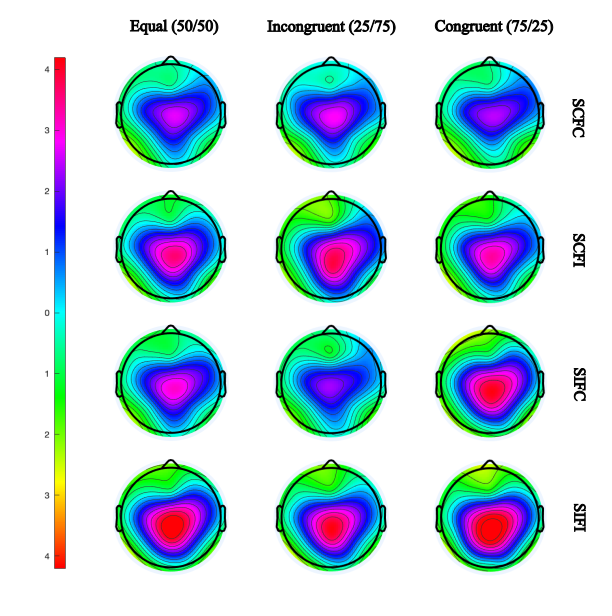
\includegraphics[width=0.25\textwidth]{scalpfig_copy}
\caption{\label{fig:latbrain} This figure was taken at 600 ms post-stimulus presentation .}
\end{wrapfigure}

Figure~\ref{fig:ERPs} This is another link to the sample data from my FYP.